In the system model, the tube cross section is sized such that the flow in the pod does not choke.
Previous models have attempted to impose this condition by assuming that the
area of the bypass flow is equal to the tube cross sectional area minus the
pod cross sectional area.\cite{Chin} This model attempts to build upon
previous models by also accounting for the development of a boundary layer over pod surface.
The boundary layer formation further reduces the bypass area and increases the
chance of choking in the flow. Thus, a larger tube will be necessary to prevent
choking when boundary layer effects are accounted for, which will increase the
costs of both raw materials and construction. This model will first analyze the
sensitivity of the tube cross sectional area to the boundary layer growth along
the pod surface. Then, estimations of boundary layer thickness as a function of
length-based $Re$ will be made in order to analyze the sensitivity of tube
cross sectional area to changes in pod length.
For each analysis, the tube is sized using the previously discussed inviscid,
quasi-1D area relationships for compressible flow. To account for the boundary
layer using this method, the boundary layer is modeled as a cylindrical ring
with a thickness equal to the maximum thickness of the displacement boundary layer,
$\delta^{*}$, over the outside of the pod, effectively reducing the area of the bypass flow.
Using this model, the contraction of the bypass flow is given by the equation
\begin{equation}
	\label{eq:epsilon}
	\varepsilon  = \frac{A_{bypass eff}}{A_{bypass}} = \frac{A_{tube}-A_{pod} -\pi  (  ( r+\delta ^{*}  )^{2}-r^{2}  )}{A_{tube}-A_{inlet}}
\end{equation}
This relationship accounts for the reduction in bypass area due to a boundary
layer of arbitrary displacement thickness. First, the sensitivity of tube area
to displacement boundary layer thickness is studied over a range of boundary
layer thicknesses for various pod cross sections. Next, the model uses a flat
plate approximation to obtain a relationship between boundary layer and length.
Since $Re > 500,000$, the boundary layer is assumed turbulent with a velocity profile \cite{FoxAndMcDonald}
\begin{equation}
	\label{eq:boundary_layer_profile}
	NEED VELOCITY PROFILE EQ
\end{equation}
Using this boundary layer velocity profile, the thickness of the displacement
boundary layer is derived using a similarity solution to produce the equation \cite{FoxAndMcDonald}
\begin{equation}
	\label{eq:boundary_layer}
	\frac{\delta^{*}}{x} \approx  \frac{.04775}{Re_{x}^{1/5}}
\end{equation}
The system model uses there to relate displacement boundary layer thickness,
and therefore tube area, with pod length. It is understood that these equations
do not accurately represent the physical relationships in our model because
they are derived in the textbook by Fox and McDonald assuming 1D flow over a
flat plate with zero pressure gradient. Characterizing the displacement
thickness of the boundary layer in 3D conical flow is beyond the scope of this analysis.
However, the approximation made in this analysis is useful for studying how
tube area and material costs may change with increasing pod length within an
order of magnitude of accuracy.  The pod configurations tested in each analysis is given in
\begin{table}
	\centering
	\caption{Configurations in boundary layer sensitivity study}
	\label{tbl:boundary_layer_sensitivty_configs}
	% \begin{tabular}
	% \end{tabular}
\end{table}
\begin{figure}
	\centering
	\caption{Tube Cross Sectional Area vs. Displacement Boundary Layer Thickness and Pod Cross Sectional Area}
	\label{fig:cross_sec_area_vs_disp_boundary_layer}
	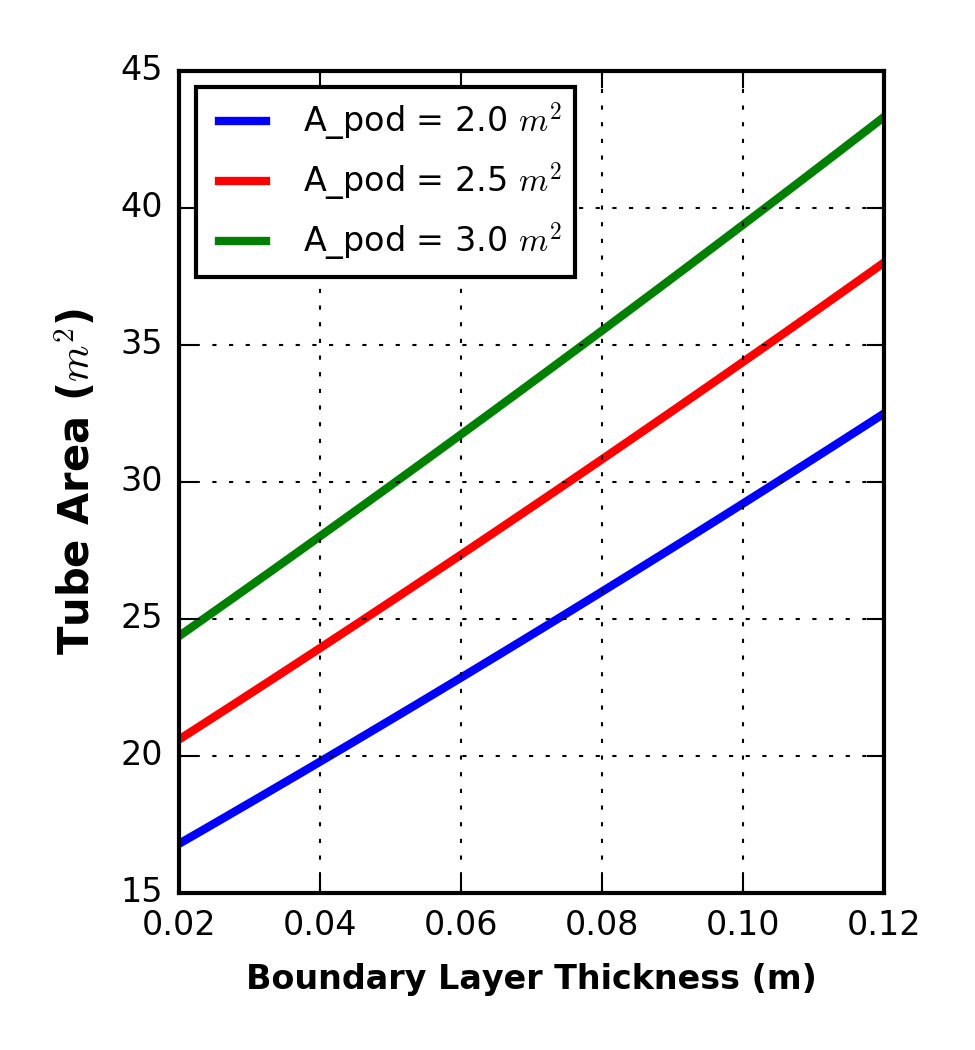
\includegraphics{../../images/graphs/boundary_layer_growth_trades/Tube_Area_vs_boundary_layer.png}
\end{figure}
\Cref{fig:cross_sec_area_vs_disp_boundary_layer} indicated the effects that
displacement boundary layer has on the cross sectional area of the tube.
It is shown that the cross sectional area of the tube increases rapidly as the
thickness of the displacement boundary layer increases.
For $A_{pod} = \SI{2d2}{\metre\squared}$, a 1 cm increase in $\delta^{*}$
results in an increase of approximately \SI{1.57}{\metre\squared} in $A_{tube}$.
Thus, it can be inferred that the tube area, and therefore the tube material cost,
are extremely sensitive to boundary layer thickness. Furthermore, the rate of
increase of the tube cross sectional area also increases with pod cross sectional area.
This relationship exists because more bypass is area is lost as pod radius
increases for a given displacement boundary layer thickness. This means that
the coupling between tube and pod cross sectional areas is even stronger than
was indicated in previous research.
\begin{figure}
	\centering
	\caption{Tube Cross Sectional Area vs. Pod Length}
	\label{fig:tube_area_vs_length}
	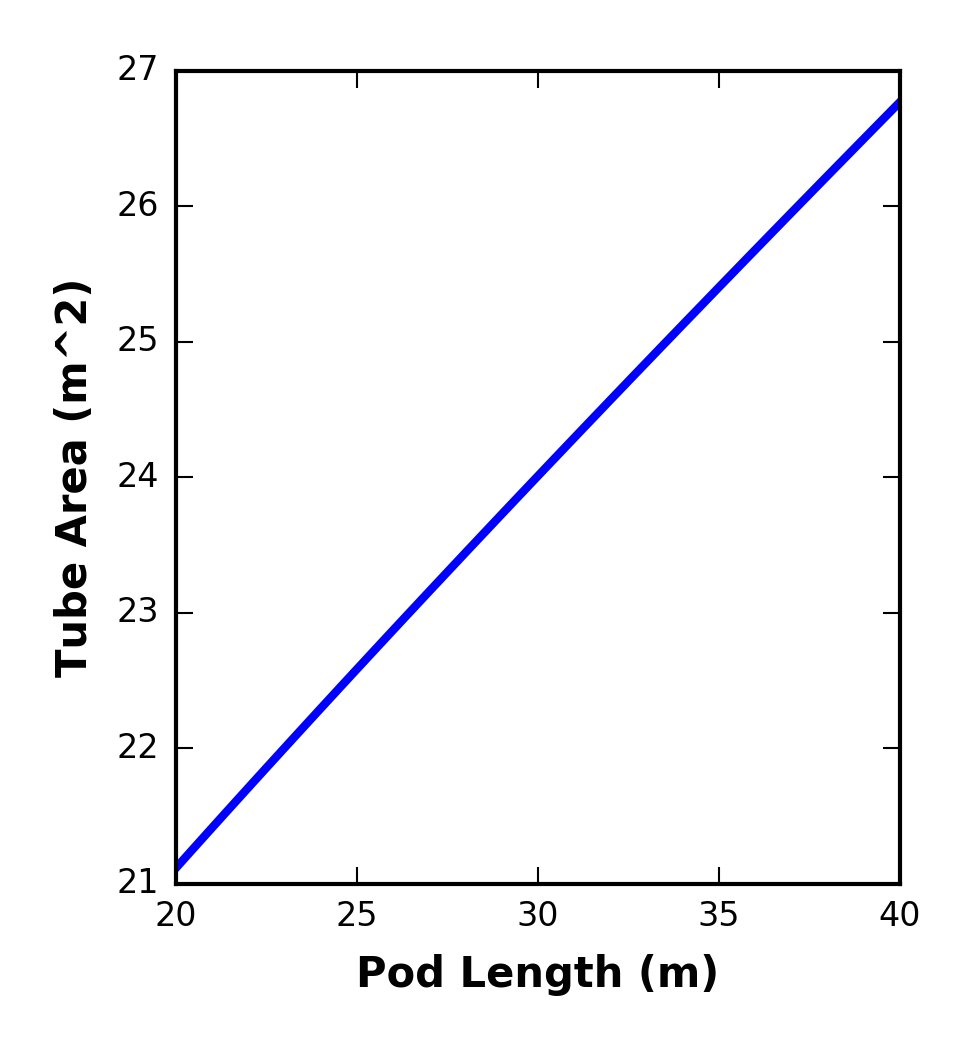
\includegraphics{../../images/graphs/boundary_layer_length_trades/Tube_Area_vs_pod_length.png}
\end{figure}
\Cref{fig:tube_area_vs_length} shows the necessary cross sectional area of the
tube as a function of pod length using the previously described relationship
approximation. It is shown that increases in pod length due to higher passenger
capacity, increased battery length, more compressor stages, etc. require the
tube cross sectional area to increase in order to accommodate for larger
boundary layer growth. This relationship reveals a coupling between tube cross
sectional area and pod length that has not been accounted for in previous system models.
The tube area is highly coupled with boundary layer thickness due to its effect on effective bypass area.
Due to the sensitivity of tube area with respect to boundary layer thickness,
it is important to develop a model that can accurately determine the
displacement boundary layer thickness over the pod surface in order to avoid
undesired choking or development of shock waves in the tube. Moreover,
this analysis suggests that active flow techniques, such as boundary layer suction,
which reduce boundary layer thickness could be very beneficial.
Since the lowest tube cross sectional area is desired for a given pod configuration,
boundary layer suction could reduce the size of the tube necessary to prevent
choking which will reduce the total material and construction costs of the system.
